\section{Обзор аналогов и формирование функциональных требований}
\label{sec:analogues}

\subsection{Steam}
\label{sec:analogues:steam}

Крупнейший сервис цифровой дистрибуции видеоигр, прошедший путь от небольшого приложения для сопровождения многопользовательских шутеров от Valve (Team Fortress Classic, Counter-Strike и Half-Life 2) в 2003 году до более чем 30 тысяч игр, одного миллиарда аккаунтов и пиком в более 20 миллионов одновременно находящихся в сети пользователей в 2020-м.
Интерфейс веб-сайта представлен на рисунке \ref*{sec:analogues:steam:layout}.

\begin{figure}[!htb]
	\centering
	  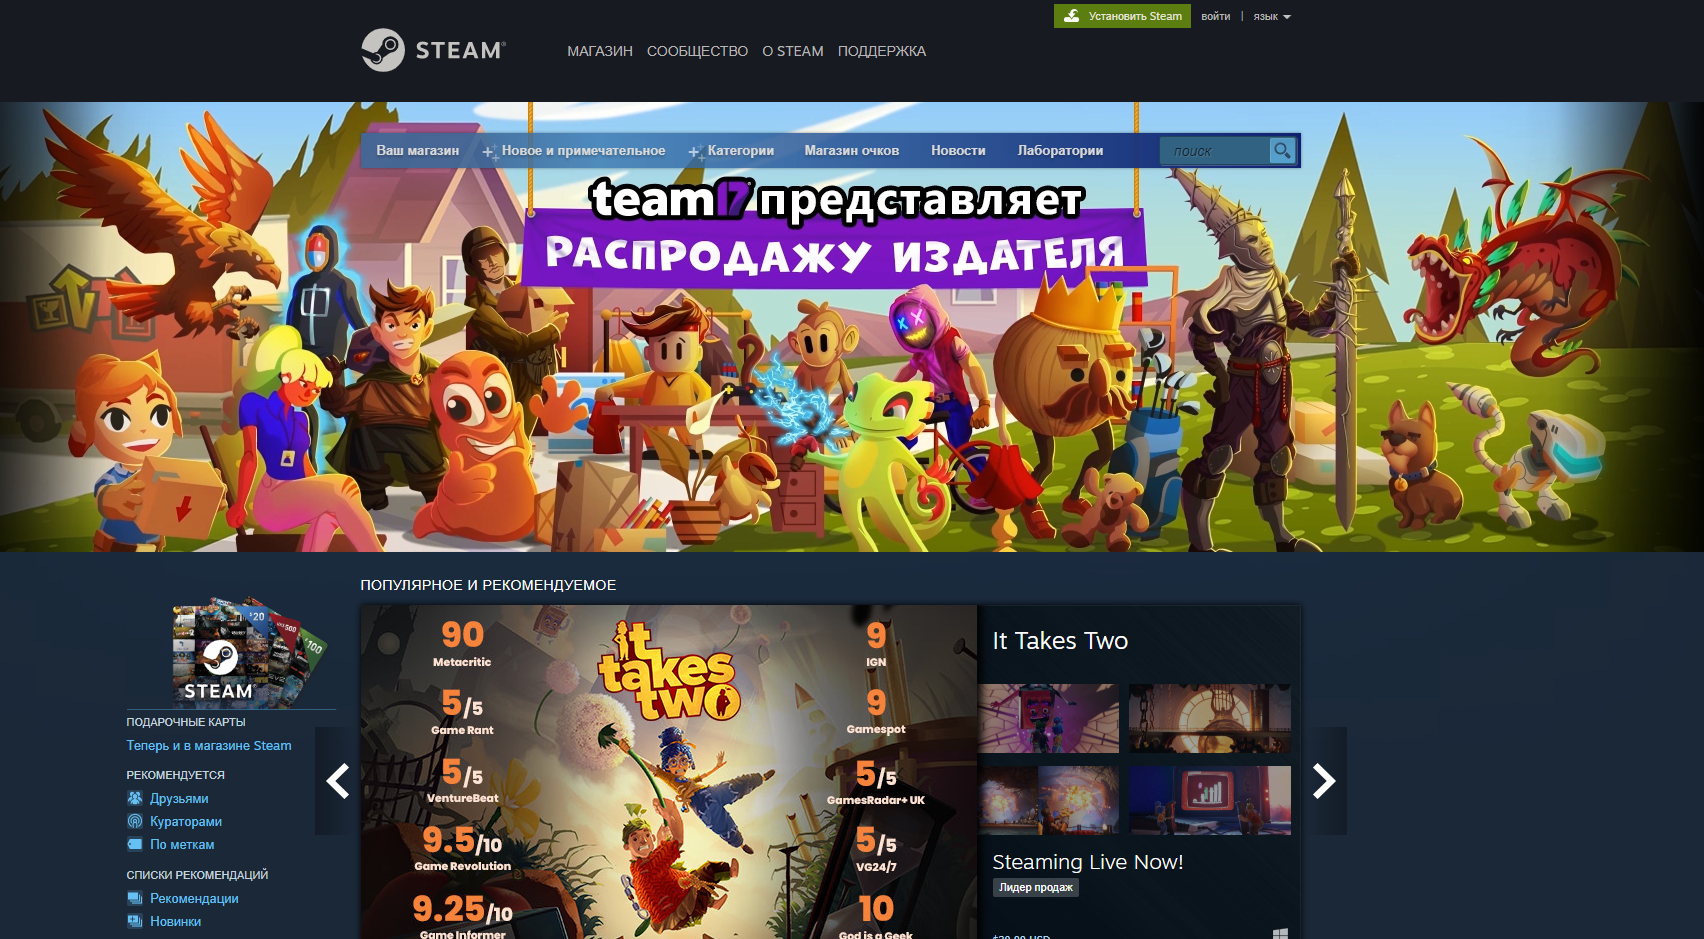
\includegraphics[scale=0.35]{attachments/steam.png}  
	  \caption{ Интерфейс веб-сайта store.steampowered.com }
	  \label{sec:analogues:steam:layout}
\end{figure}

Такая аудитория досталась магазину благодаря упорному труду на протяжении многих лет его развития. Valve вкладывает огромные ресурсы в разработку Steam, за счет чего его можно назвать не просто сервисом, а целой социальной сетью для игроков: с магазином и библиотекой игр, списком друзей и чатом, пользовательскими отзывами, обсуждениями и трансляциями, руководствами и скриншотами, пользовательскими дополнениями и торговой площадкой, достижениями, карточками и кастомизацией профилей.

Сервис предлагает, пожалуй, самые комфортные условия для клиентов. В каталоге игр присутствует удобный поиск по жанрам, тегам, популярности и другим критериям, разработчики могут устанавливать региональные цены, а сами цены представлены в самых разных валютах, начиная от американского доллара и российского рубля, заканчивая мексиканским песо и вьетнамским донгом. Поддерживаются и различные способы оплаты, включая банковские карты и внутренний кошелек Steam, который можно пополнить посредством многих платежных систем.

Впрочем, есть у сервиса и недостатки. Так, крайне свободная политика Valve относительно публикации игр в Steam и почти полное отсутствие цензуры привели к появлению на платформе большого количества низкокачественных продуктов. Кроме того, некоторым пользователям не нравится неповоротливость Valve в плане развития магазина: компания слишком редко добавляет интерфейсные изменения в клиент и почти не реагирует на действия конкурентов.

\subsection{Epic Games Store}
\label{sec:analogues:egs}

Относительно молодой (запущен в декабре 2018 года), но уже обративший на себя внимание сервис от компании Epic Games. Все из-за неоднозначной политики создателей: с самого момента появления сервиса, он постоянно фигурирует в различных скандалах. Это и покупка эксклюзивности игр с изъятием их из Steam, и информация о сканировании приложением Epic Games Launcher (являющимся, по совместительству и магазином, и библиотекой игр) папок Steam, и распродажа, в ходе которой издатели снимали с продажи свои игры.
Интерфейс веб-сайта представлен на рисунке \ref*{sec:analogues:egs:layout}.

\begin{figure}[!htb]
	\centering
	  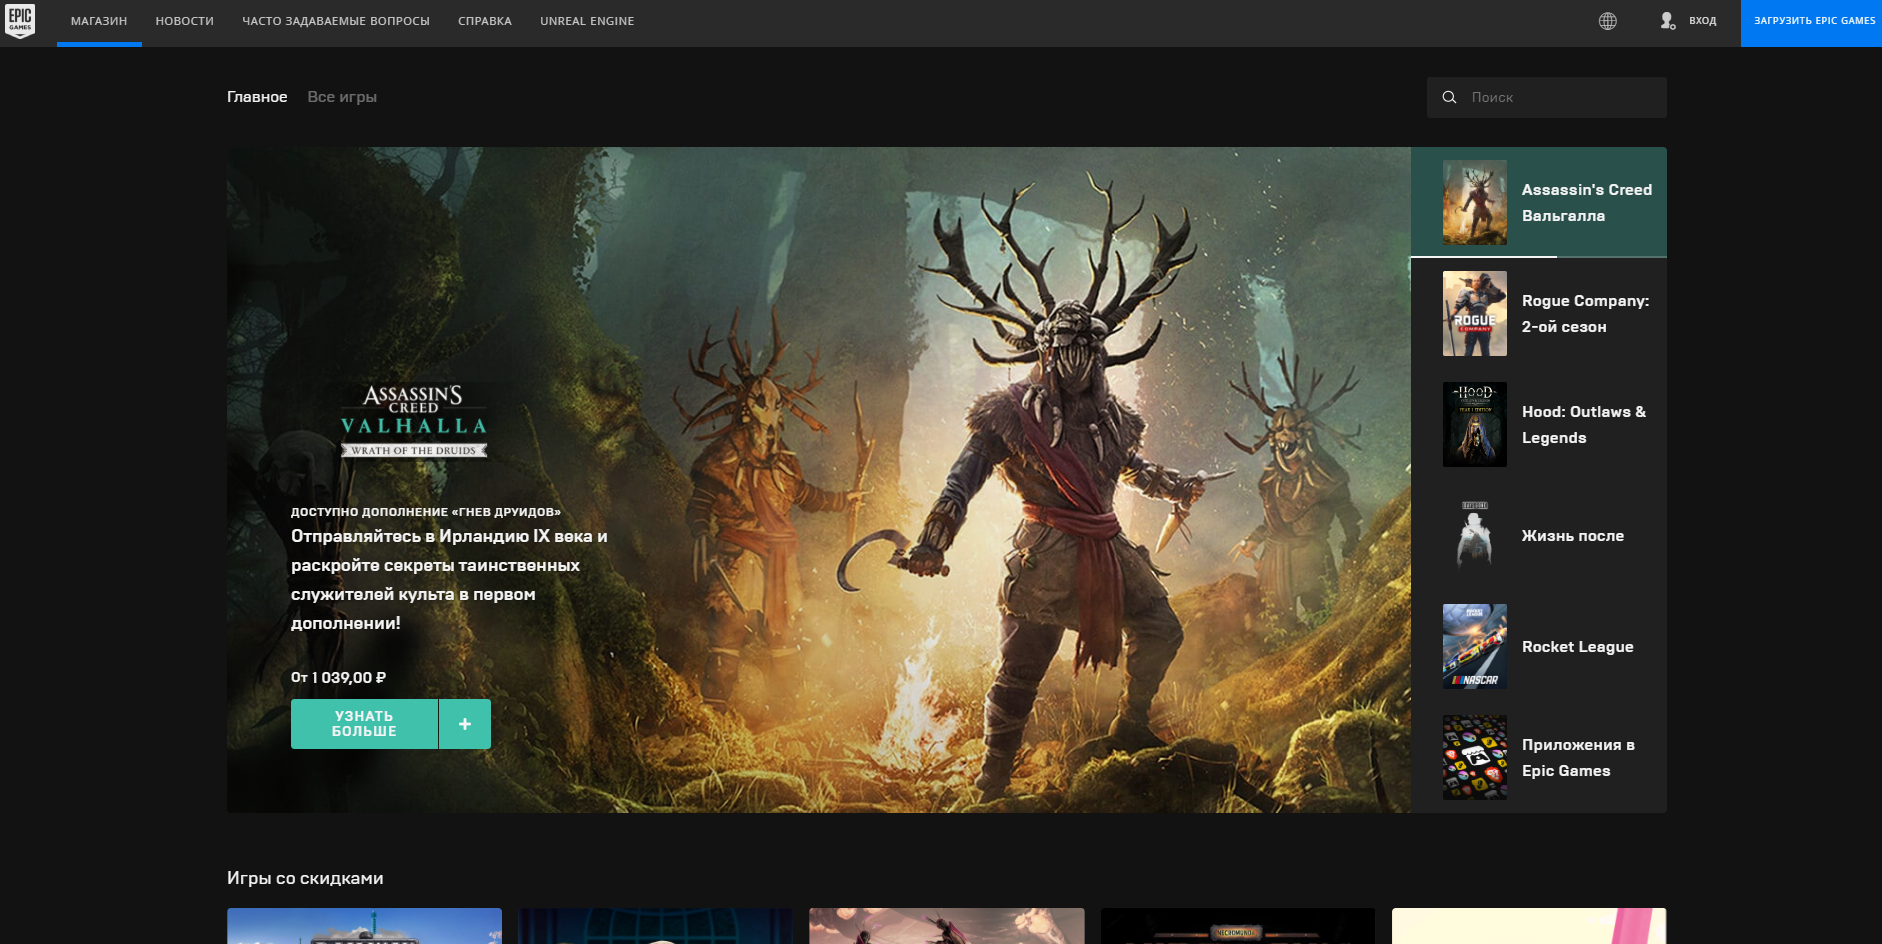
\includegraphics[scale=0.3]{attachments/egs.png}  
	  \caption{ Интерфейс веб-сайта epicgames.com }
	  \label{sec:analogues:egs:layout}
\end{figure}

Так как сервис ещё очень молод, он не обладает каким-то внушительным функционалом, однако есть несколько преимуществ, выгодно выделяющих его на уровне конкурентов: во-первых, из-за низкой комиссии, многие разработчики выставляют свои видеоигры экслюзивно в Epic Games; во-вторых, на сервисе бывают гораздо более выгодные по сравнению с конкурентами предложения.

Однако сервис имеет и несколько недостатков, самыми существенными из которых являются его медленная работа, отсутствие корзины и невозможность оставлять и читать отзывы других покупателей.

\subsection{Origin}
\label{sec:analogues:origin}

Сервис Origin был запущен компанией Electronic Arts в 2011 году: издатель хотел собирать продавать издаваемые им игры единолично, не делясь прибылью с владельцами других сервисов (до старта Origin игры от ЕА издавались в Steam).
Интерфейс веб-сайта представлен на рисунке \ref*{sec:analogues:origin:layout}.

\begin{figure}[!htb]
	\centering
	  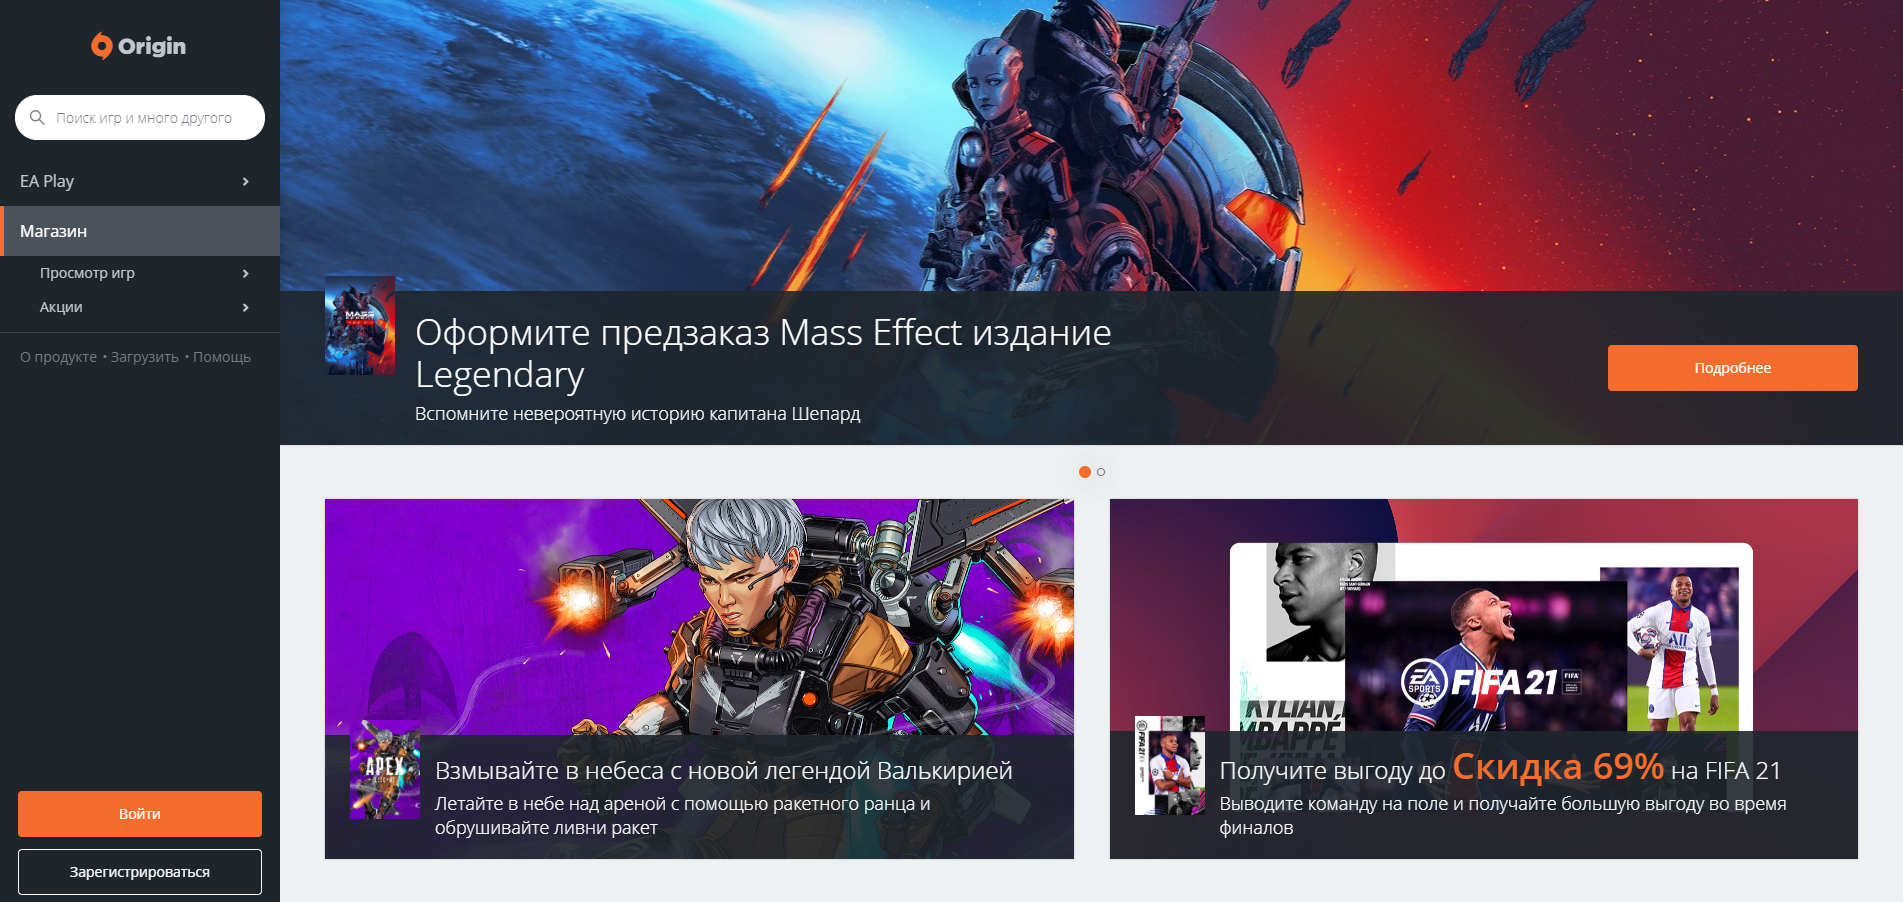
\includegraphics[scale=0.3]{attachments/origin.png}  
	  \caption{ Интерфейс веб-сайта origin.com }
	  \label{sec:analogues:origin:layout}
\end{figure}

Сервис предлагает большую часть функционала, присутствующего у конкурентов: оплатить покупки можно с помощью распространенных платежных систем, а для пользователей из разных частей мира действуют региональные цены. Кроме того, ЕА регулярно проводит распродажи и бесплатные раздачи видеоигр. Присутствуют и социальные функции: список друзей и чат, автообновления игр, но по их количеству сервис все же не дотягивает до Steam.

Основными недостатками сервиса являются отсутствие возможности оставлять и просматривать отзывы покупателей, небольшой каталог видеоигр и медленная работа.

\subsection{Формирование функциональных требований}
\label{sec:analogues:requirements}

Проанализировав существующие на рынке сервисы цифровой дистрибуции видеоигр, можно сделать вывод, что разрабатываемый сервис должен обладать следующими функциями:
\begin{itemize}
	\item Наличие корзины, позволяющей приобрести несколько видеоигр за раз.
	\item Фильтрация каталога видеоигр по названию, жанру, цене.
	\item Возможность смены локализации сервиса: русский либо английский язык на выбор.
	\item Возможность восстановить доступ к аккаунту в случае утери пароля или электронной почты.
	\item Возможность оставлять и просматривать отзывы пользователей о видеоиграх.
\end{itemize} 
